\documentclass{standalone}
\usepackage{tikz}
\usetikzlibrary{3d}
\usetikzlibrary{backgrounds}
\usetikzlibrary{arrows,calc}
%
\usepackage{xcolor}
%
\definecolor{space}{HTML}{1F2C4E}
\definecolor{earth}{HTML}{0089FA}

\title{Campo magnetico}
\begin{document}
	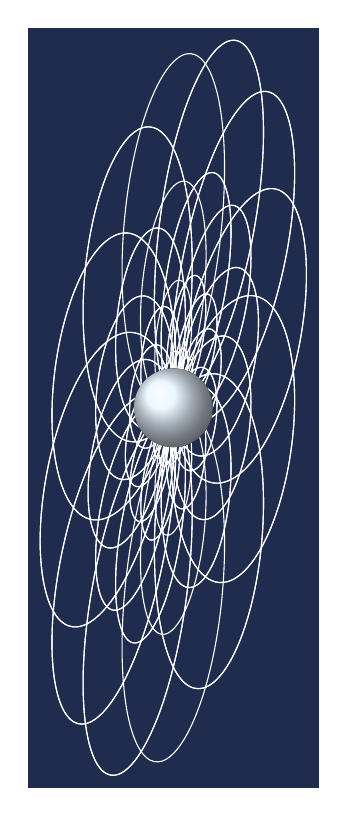
\begin{tikzpicture}[scale=1.0,background rectangle/.style={fill=space},show background rectangle,
		%Option for nice arrows%
		>=latex,%
		inner sep=0pt,%
		outer sep=2pt,%
		mark coordinate/.style={outer sep=0pt,
			minimum size=3pt, fill=black,circle}%
		]
		%% some definitions
		\def\R{0.5}       % sphere radius
		\def\angEl{30}    % elevation angle
		\def\angAz{-140}  % azimuth angle
		\def\angPhi{-105} % longitude of point
		\def\angBeta{55}  % latitude of point
		\def\angGam{-190} % longitude of point
		%% working planes
		\pgfmathsetmacro\H{\R*cos(\angEl)}          % Distance to north pole
		%\LongitudePlane[xzplane]{\angEl}{\angAz}    % x-axis plane
		%
		\coordinate (O) at (0,0);
		%
	%\draw[line width=1pt,->] (-4,0) -- (4,0);
	%\draw[line width=1pt,->] (0,-4) -- (0,4);
	
	%\foreach \ang in {0,30,...,360}
	%	\begin{scope}[rotate around={\ang:(0,0)}]
			
	%	\end{scope}
	
	\begin{scope}[canvas is zy plane at x=0]
		\foreach \ang in {30,60,...,330}
		\foreach \u in {0,...,5}
		\draw[color=white,domain=-3.14:3.14,samples=200,smooth,rotate=\ang] plot (canvas polar cs:angle=\x r,radius={\u*sin(\x r)*\u*sin(\x r)*5});
	\end{scope}
		
	\fill[ball color=earth!10] (0,0) circle (\R);

	\end{tikzpicture}
\end{document}